% SC3270 --- Chapter 3: Invariants - What Stays True (0->100 ground-up)
\chapter{Invariants: What Stays True}
\label{ch:invariants}

\begin{quote}
\emph{``An invariant is the sentence a loop keeps repeating to itself so it does not get lost.''} Find that sentence and you can prove the loop correct without unrolling it infinitely.
\end{quote}

\noindent\fbox{\parbox{\dimexpr\linewidth-2\fboxsep-2\fboxrule}{%
\textbf{From zero: no invariant experience assumed.} We define invariants from scratch, show how to discover them by splitting what is done from what remains, and practise judging too-weak and too-strong candidates. Pictures guide every definition; formalism follows.}}
\vspace{0.4em}

\section*{Learning Outcomes}
After this chapter you will be able to:
\begin{enumerate}[label=(L\arabic*)]
    \item define invariant (loop, data, class) and state its preservation condition;
    \item propose an invariant for a simple loop by done/remaining decomposition;
    \item check that invariant $\land$ $\neg$guard implies postcondition;
    \item diagnose invariants that are too weak or too strong;
    \item explain why invariants are the induction hypothesis of a loop.
\end{enumerate}

% ============================================================
\section{What Is an Invariant?}
\label{sec:what-invariant}
\paragraph{Intuition.} Watch someone sorting a hand of cards by insertion: after each insertion, the left portion is sorted. That sortedness never breaks—it is \emph{invariant} across iterations. If you know what stays sorted and what remains unsorted, you understand the whole algorithm without watching every swap.

A loop invariant is a \emph{property of the state} that is true before the loop, stays true after each iteration, and—together with the loop having exited—implies the desired postcondition. Three obligations:
\[
\text{(init)}\; P\Rightarrow I \qquad \text{(preserve)}\; \{I\land B\}\;C\;\{I\} \qquad \text{(exit)}\; I\land\neg B\Rightarrow Q.
\]

\begin{figure}[h]\centering
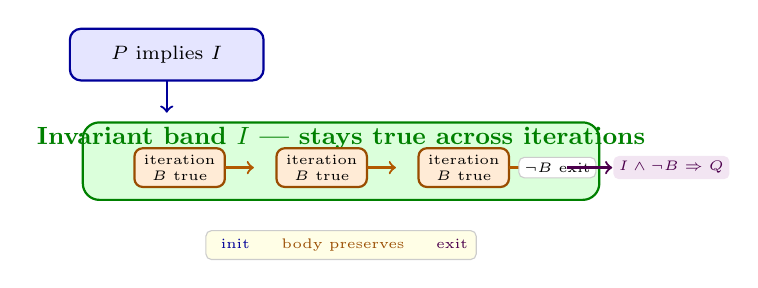
\begin{tikzpicture}[scale=0.82,font=\scriptsize]
\draw[fill=blue!10,draw=blue!60!black,thick,rounded corners=4pt] (0,2.2) rectangle (3.0,3.0);
\node at (1.5,2.60) {$P$ implies $I$};
\draw[->,thick,blue!60!black] (1.5,2.20) -- (1.5,1.70);
\draw[fill=green!14,draw=green!50!black,thick,rounded corners=6pt] (0.2,0.35) rectangle (8.2,1.55);
\node[font=\small\bfseries,green!50!black] at (4.2,1.30) {Invariant band $I$ --- stays true across iterations};
\foreach \x in {1.0,3.2,5.4} {
  \draw[fill=orange!16,draw=orange!60!black,thick,rounded corners=3pt] (\x,0.55) rectangle (\x+1.4,1.15);
  \node[font=\tiny,align=center] at (\x+0.70,0.85) {iteration\\ $B$ true};
  \draw[->,thick,orange!70!black] (\x+1.40,0.85) -- (\x+1.85,0.85);
}
\node[font=\tiny,fill=white,draw=gray!40,rounded corners=2pt,inner sep=2pt] at (7.55,0.85) {$\neg B$ exit};
\draw[->,thick,violet!60!black] (7.70,0.85) -- (8.4,0.85) node[right,font=\tiny,fill=violet!10,rounded corners=2pt,inner sep=2pt] {$I\land\neg B\Rightarrow Q$};
\node[font=\tiny,align=left,fill=yellow!10,draw=gray!40,rounded corners=2pt,inner sep=3pt] at (4.2,-0.35) {\textcolor{blue!60!black}{$\blacksquare$ init} \quad \textcolor{orange!60!black}{$\blacksquare$ body preserves} \quad \textcolor{violet!60!black}{$\blacksquare$ exit}};
\end{tikzpicture}
\caption{Invariant as a fence: you enter inside $I$ (init), each lap stays inside (preserve), and leaving through the $\neg B$ gate lands in $Q$.}
\label{fig:invariant-fence}
\end{figure}

Like induction, the invariant is the \emph{induction hypothesis} for loops: base case is $P\Rightarrow I$, inductive step is $\{I\land B\}\,C\,\{I\}$, conclusion is $I\land\neg B\Rightarrow Q$.

\begin{figure}[h]\centering
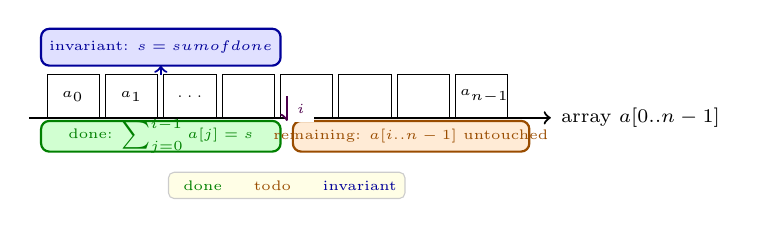
\begin{tikzpicture}[scale=0.78,font=\scriptsize]
\draw[->,thick] (0,0) -- (8.5,0) node[right] {array $a[0..n-1]$};
\foreach \i in {0,1,2,3,4,5,6,7} \draw (\i*0.95+0.3,0) rectangle (\i*0.95+1.15,0.70);
\node[font=\tiny] at (0.72,0.35) {$a_0$}; \node[font=\tiny] at (1.67,0.35) {$a_1$};
\node[font=\tiny] at (2.62,0.35) {$\dots$}; \node[font=\tiny] at (7.42,0.35) {$a_{n-1}$};
\draw[fill=green!18,draw=green!50!black,thick,rounded corners=3pt] (0.20,-0.55) rectangle (4.10, -0.05);
\node[font=\tiny,green!50!black] at (2.15,-0.30) {done: $\sum_{j=0}^{i-1} a[j]=s$};
\draw[fill=orange!16,draw=orange!60!black,thick,rounded corners=3pt] (4.30,-0.55) rectangle (8.15,-0.05);
\node[font=\tiny,orange!60!black] at (6.22,-0.30) {remaining: $a[i..n-1]$ untouched};
\draw[fill=blue!12,draw=blue!60!black,thick,rounded corners=3pt] (0.20,0.85) rectangle (4.10,1.45);
\node[font=\tiny,blue!60!black] at (2.15,1.15) {invariant: $s = \text{sum of done}$};
\draw[->,thick,blue!60!black] (2.15,0.70) -- (2.15,0.85);
\draw[->,thick,violet!60!black] (4.2,0.35) -- (4.2,-0.05) node[midway,right,font=\tiny,fill=white] {$i$};
\node[font=\tiny,align=left,fill=yellow!10,draw=gray!40,rounded corners=2pt,inner sep=3pt] at (4.2,-1.10) {\textcolor{green!50!black}{$\blacksquare$ done} \quad \textcolor{orange!60!black}{$\blacksquare$ todo} \quad \textcolor{blue!60!black}{$\blacksquare$ invariant}};
\end{tikzpicture}
\caption{Discovery pattern for summation: $I\equiv 0\le i\le n\land s=\sum_{j=0}^{i-1}a[j]$. Done plus todo equals whole job.}
\label{fig:done-todo}
\end{figure}

% ============================================================
\section{Discovering Invariants: Done vs.\ Remaining}
\label{sec:discovery}
A reliable recipe: ask \emph{what has the loop achieved so far?} and \emph{what is left?} The invariant ties the two to the final goal.

\textbf{Summation:} $s:=0;\;i:=0;\;\texttt{while }i<n\texttt{ do }s:=s+a[i];\;i:=i+1$ with $\{ \text{true}\}\,\dots\,\{s=\sum_{j=0}^{n-1}a[j]\}$. Done $=\sum_{j < i}$, remaining $= \sum_{j\ge i}$. So propose $I\equiv 0\le i\le n \land s=\sum_{j=0}^{i-1}a[j]$. Check: init $i=0\Rightarrow s=0=\sum_{\emptyset}=0$. Preserve: adding $a[i]$ shifts done by one. Exit $i=n\Rightarrow s=\sum_{j=0}^{n-1}a[j]=Q$.

\begin{lstlisting}[language=Python, caption={Summation with invariant as executable assertion: fails loudly if discovery is wrong.}, label={lst:sum-invariant}]
def sum_array(a):
    s, i, n = 0, 0, len(a)
    # I: 0<=i<=n and s == sum(a[0:i])
    assert 0 <= i <= n and s == sum(a[0:i])
    while i < n:
        # I and B (i<n) hold
        s += a[i]; i += 1
        assert 0 <= i <= n and s == sum(a[0:i])  # I preserved
    # I and not B (i==n) => s == sum(a)
    assert s == sum(a)
    return s
\end{lstlisting}

\textbf{Counting positives:} $c:=0;\;i:=0;\;\texttt{while }i<n\texttt{ do if }a[i]>0\texttt{ then }c:=c+1;\;i:=i+1$ yields $I\equiv 0\le i\le n\land c = |\{j < i : a[j]>0\}|$.

% ============================================================
\section{Too Weak, Too Strong, Just Right}
\label{sec:weak-strong}
An invariant can fail two ways:

\textbf{Too weak:} $\{ \text{true}\}\,C\,\{Q\}$ holds for any $C$ but does not imply $Q$ at exit. Example: $I\equiv 0\le i\le n$ for summation—preserved, but $I\land i=n$ says only $i=n$, not $s$'s value. So $I\land\neg B\not\Rightarrow Q$.

\textbf{Too strong:} $I\equiv s=\sum_{j=0}^{i-1}a[j]\land i=n$ claims the loop is already done before it starts—init fails because $0=n$ is false unless $n=0$.

Goldilocks $I$ is strong enough to imply $Q$ at exit, weak enough to be established initially and preserved. Strengthening a weak $I$ (add the $s$ conjunct) or weakening a strong $I$ (drop $i=n$) moves toward the sweet spot.

\begin{figure}[h]\centering
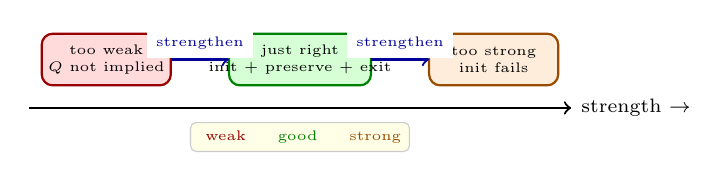
\begin{tikzpicture}[scale=0.82,font=\scriptsize]
\draw[->,thick] (0,0) -- (8.4,0) node[right] {strength $\to$};
\draw[fill=red!14,draw=red!60!black,thick,rounded corners=4pt] (0.2,0.35) rectangle (2.2,1.15);
\node[font=\tiny,align=center] at (1.20,0.75) {too weak\\ $Q$ not implied};
\draw[fill=green!16,draw=green!50!black,thick,rounded corners=4pt] (3.1,0.35) rectangle (5.3,1.15);
\node[font=\tiny,align=center] at (4.20,0.75) {just right\\ init + preserve + exit};
\draw[fill=orange!14,draw=orange!60!black,thick,rounded corners=4pt] (6.2,0.35) rectangle (8.2,1.15);
\node[font=\tiny,align=center] at (7.20,0.75) {too strong\\ init fails};
\draw[->,thick,blue!60!black] (2.20,0.75) -- (3.10,0.75) node[midway,above,font=\tiny,fill=white] {strengthen};
\draw[->,thick,blue!60!black] (5.30,0.75) -- (6.20,0.75) node[midway,above,font=\tiny,fill=white] {strengthen};
\node[font=\tiny,fill=yellow!10,draw=gray!40,rounded corners=2pt,inner sep=3pt] at (4.2,-0.45) {\textcolor{red!60!black}{$\blacksquare$ weak} \quad \textcolor{green!50!black}{$\blacksquare$ good} \quad \textcolor{orange!60!black}{$\blacksquare$ strong}};
\end{tikzpicture}
\caption{Invariant strength spectrum: weak cannot reach $Q$, strong cannot be entered, just-right does both.}
\label{fig:weak-strong}
\end{figure}

\begin{lstlisting}[language=C, caption={Three candidates for summation---only one survives all three checks.}, label={lst:weak-strong-c}]
// Candidate A (too weak):  0<=i<=n
//   preserve OK, but upon exit i==n does NOT imply s==sum(a)

// Candidate B (just right): 0<=i<=n && s==sum(a[0..i-1])
//   init: i=0,s=0 OK; preserve: s+=a[i],i++ OK; exit: i==n => s==sum(a)

// Candidate C (too strong): s==sum(a[0..i-1]) && i==n
//   init fails when n>0: i==n is false at start
\end{lstlisting}

\begin{example}[Linear search invariant]
$a[0..n-1]$, search $key$, $i:=0;\texttt{while }i<n\land a[i]\neq key\texttt{ do }i:=i+1$. Good invariant: $I\equiv 0\le i\le n\ \land\ (\forall j<i.\,a[j]\neq key)$. Then $I\land\neg(i<n\land a[i]\neq key)$ splits into $i=n\lor a[i]=key$, and $I$ tells us no earlier position held $key$—exactly the post we want.
\end{example}

% ============================================================
\section{Why Invariants Suffice: Induction Over Iterations}
\label{sec:induction}
Unrolling a loop yields a sequence of states $\sigma_0,\sigma_1,\dots$ where $\sigma_{k+1}$ is after $k+1$ iterations. The preservation condition $\{I\land B\}\,C\,\{I\}$ says: if $\sigma_k\models I\land B$ then $\sigma_{k+1}\models I$. By induction on $k$, every reachable $\sigma_k\models I$. So $I$ holds no matter how many times we go around. At exit we additionally know $\neg B$, and $I\land\neg B\Rightarrow Q$ transfers truth to the post.

This is why invariants beat testing: testing checks finitely many $\sigma_k$; induction covers \emph{all} $k$, including the largest $n$ that triggers overflow, aliasing, or off-by-one that a test suite likely misses.

\begin{example}[Off-by-one caught]
Program: $i:=0;\,s:=0;\;\texttt{while }i<n\texttt{ do }s:=s+a[i];\,i:=i+1$ but writer forgets $i:=i+1$. Invariant $I\equiv 0\le i\le n\land s=\sum_{j<i}a[j]$ is not preserved: after one body execution $i$ unchanged, so $s$ becomes $s+a[i]$ while $i$ still old, breaking $s=\sum_{j<i}a[j]$. The preservation VC $I\land i<n\Rightarrow \text{wp}(s:=s+a[i];\,I)$ fails—proof catches the missing increment statically.
\end{example}

\begin{remark}[Data invariants vs loop invariants]
A \emph{data invariant} holds between method calls (e.g., ``list is sorted''); a \emph{loop invariant} holds between iterations. Both are preserved by a step, but scope differs. A class invariant broken inside a method is fine provided it is re-established before return, just as a loop invariant may be broken mid-body provided it is restored by the iteration's end.
\end{remark}

% ============================================================
\section{Inventing vs.\ Checking}
\label{sec:invent-check}
Finding $I$ is creative; checking it is mechanical. In modern verifiers (Dafny, Why3) you \emph{supply} $I$ and the tool generates VCs $P\Rightarrow I$, $I\land B\Rightarrow \text{wp}(C,I)$, $I\land\neg B\Rightarrow Q$ and discharges them with an SMT solver. So skill splits: human invents the shape (done/remaining), machine checks the details.

Heuristic checklist: (1) include bounds $0\le i\le n$—almost always needed; (2) state what done means with quantifiers; (3) ensure $I$ mentions every variable the loop mutates; (4) test $I$ on $i=0$ (init) and $i=n$ (exit) before proving preserve.

% ============================================================
\section{Worked Mini-Proof: Summation End-to-End}
\label{sec:mini-proof-sum}
Claim: $\{ n\ge0\}\; s:=0;i:=0;\;\texttt{while }i<n\texttt{ do }(s:=s+a[i];i:=i+1)\; \{s=\sum_{j=0}^{n-1}a[j]\}$.

Take $I\equiv 0\le i\le n\land s=\sum_{j=0}^{i-1}a[j]$. Show:

\textit{Init:} From $s=0,i=0$ we have $0\le0\le n$ and $\sum_{j=0}^{-1}a[j]=0$ (empty sum), so $I$.

\textit{Preserve:} Assume $I\land i<n$, i.e.\ $0\le i<n\land s=\sum_{j=0}^{i-1}a[j]$. After $s':=s+a[i]$ we have $s'=\sum_{j=0}^{i}a[j]$; after $i':=i+1$ we have $s'=\sum_{j=0}^{i'-1}a[j]$ and $0\le i'\le n$. So $I$ restored.

\textit{Exit:} $I\land i\ge n$ gives $i=n$ (from $0\le i\le n$) and thus $s=\sum_{j=0}^{n-1}a[j]=Q$.

Every step uses only substitution and arithmetic; no loop unrolling needed. That is the power: one invariant replaces infinitely many iteration cases. The same template works for product, count, and search—only the done conjunct changes.

\begin{remark}[Empty sum convention]
Define $\sum_{j=0}^{-1}a[j]=0$ so the base case $i=0$ holds uniformly. For product use $1$; for $\forall j<i.\,P(j)$ use $\text{true}$ when $i=0$. Consistent base values make $P\Rightarrow I$ trivial.
\end{remark}

% ============================================================
\section{Exercises}
\label{sec:ch03-exercises}
\begin{enumerate}[label=E3.\arabic*, leftmargin=*, itemsep=0.6em]
    \item \textbf{Propose and test.} Give $I$ for counting zeros in $a[0..n-1]$ and check the three conditions $P\Rightarrow I$, $\{I\land B\}\,C\,\{I\}$, $I\land\neg B\Rightarrow Q$.
    \item \textbf{Too weak diagnosis.} Show $I\equiv 0\le i\le n$ for the positivity counter is preserved but fails to imply $c=|\{j<n:a[j]>0\}|$ at exit. What minimal conjunct fixes it?
    \item \textbf{Too strong diagnosis.} Show $I\equiv c=|\{j<i:a[j]>0\}|\land i=n$ fails at init when $n>0$. Weaken it minimally to a correct invariant.
    \item \textbf{Search invariant.} Prove that $I\equiv \forall j<i.\,a[j]\neq key$ for linear search implies the post $(r=-1\Rightarrow\forall j.\,a[j]\neq key)\land(r\ge0\Rightarrow a[r]=key)$.
    \item \textbf{Done/remaining for product.} Write $I$ for $p:=\prod_{j=0}^{i-1} a[j]$ and verify preserve step uses the substitution axiom for $p:=p*a[i]$.
\end{enumerate}

\section*{Chapter Notes}
The done/remaining heuristic is folklore in Gries, \emph{The Science of Programming} (1981). Invariants as induction hypotheses appear in Floyd (1967) and Hoare (1969). For practice, annotate every loop you write this week with its invariant—even when not required to prove it.

\smallskip
\begin{remark}[Mental trick]
Before coding a loop, write $I$ and $Q$ first, then derive the guard as ``not yet $Q$'' and the body as ``make progress toward $Q$ while preserving $I$''. This is correctness by construction in miniature—Chapter~8 scales it to whole programs.
\end{remark}
% End of Chapter 3
